\documentclass[12pt,a4paper]{article}
\usepackage[margin=2.5cm]{geometry}
\usepackage{amsmath,amssymb}
\usepackage{booktabs}
\usepackage{array}
\usepackage{enumitem}
\usepackage{parskip}
\usepackage[T1]{fontenc}
\usepackage{times}
\usepackage{tikz}
\usetikzlibrary{positioning,arrows.meta}

\setlength{\parindent}{0pt}
\setlength{\parskip}{6pt}
\setlist[itemize]{noitemsep,topsep=2pt,leftmargin=1.4em,label={--}}
\setlist[enumerate]{noitemsep,topsep=2pt,leftmargin=1.8em}

\begin{document}

\begin{center}
{\Large\textbf{IE 400 -- Term Project Report}}\\[4pt]
Spring 2026\\[8pt]
\textbf{Berke \.{I}smail Erhan As{\i}l} \quad (22203732)\\[2pt]
\textbf{Halis Vefa T\"{u}rky{\i}lmaz} \quad (22102898)\\[2pt]
\textbf{Aziz \"{U}z\"{u}mc\"{u}} \quad (22102800)
\end{center}

\bigskip

%=======================================================================
\section*{\underline{Question 1: Museum Escape}}

\subsection*{Problem Definition}

Lara starts at cell $(1,1)$ and must reach the exit at cell $(8,8)$ on an $8\times8$ grid
in the minimum number of time steps. At each time step she may move one cell up, down,
left or right or stay in place. She cannot enter obstacle cells. Three security cameras
patrol the museum; if Lara occupies any camera visible cell at the same time step, she is
caught.

\textbf{Obstacle cells:}
$(1,3),\,(2,2),\,(2,5),\,(3,7),\,(4,2),\,(4,3),\,(5,5),\,(6,4),\,(7,1),\,(7,4),\,(7,5)$

\subsection*{Camera Movement Tables}

\textbf{Camera 1}:

\begin{center}
\begin{tabular}{cccc}
\toprule
$t$ & Position & Direction & Visible Cells \\
\midrule
0   & $(3,3)$ & Right & $(3,3),(3,4),(3,5)$ \\
1   & $(3,4)$ & Right & $(3,4),(3,5),(3,6)$ \\
2   & $(3,5)$ & Left  & $(3,5),(3,4),(3,3)$ \\
3   & $(3,4)$ & Left  & $(3,4),(3,3),(3,2)$ \\
$4+$ & \multicolumn{3}{l}{repeats from $t=0$} \\
\bottomrule
\end{tabular}
\end{center}

\textbf{Camera 2}:

\begin{center}
\begin{tabular}{cccc}
\toprule
$t$ & Position & Direction & Visible Cells \\
\midrule
0 & $(4,6)$ & Down  & $(4,6),(5,6)$ \\
1 & $(5,6)$ & Down  & $(5,6),(6,6)$ \\
2 & $(6,6)$ & Right & $(6,6),(6,7)$ \\
3 & $(6,7)$ & Left  & $(6,7),(6,6)$ \\
4 & $(6,6)$ & Up    & $(6,6),(5,6)$ \\
5 & $(5,6)$ & Up    & $(5,6),(4,6)$ \\
$6+$ & \multicolumn{3}{l}{repeats from $t=0$} \\
\bottomrule
\end{tabular}
\end{center}

\textbf{Camera 3}:

\begin{center}
\begin{tabular}{cccc}
\toprule
$t$ & Position & Direction & Visible Cells \\
\midrule
0 & $(7,7)$ & NE & $(7,7),(6,8)$ \\
1 & $(6,8)$ & SW & $(6,8),(7,7),(8,6)$ \\
2 & $(7,7)$ & SW & $(7,7),(8,6)$ \\
3 & $(8,6)$ & SW & $(8,6),(7,7),(6,8)$ \\
$4+$ & \multicolumn{3}{l}{repeats from $t=0$} \\
\bottomrule
\end{tabular}
\end{center}

The combined camera visible set at time $t$ is
\[
  F(t) = C_1[t \bmod 4]\;\cup\; C_2[t \bmod 6]\;\cup\; C_3[t \bmod 4].
\]

%-----------------------------------------------------------------------
\subsection*{Task 1: Integer Programming Formulation}

\textbf{Sets and Parameters}
\begin{itemize}
  \item $\mathcal{V}$: set of all non-obstacle cells $(r,c)$, where $r,c\in\{1,\ldots,8\}$
  \item $N(r,c)$: set of cells reachable in one step from $(r,c)$, including $(r,c)$ itself
        and its orthogonal neighbours in $\mathcal{V}$
  \item $F(t)$: set of cells visible by any camera at time $t$
  \item $T_{\max}=30$: maximum planning horizon (an upper bound on the number of steps)
\end{itemize}

\textbf{Decision Variables}
\[
  x_{t,r,c} \in \{0,1\} \qquad t=0,1,\ldots,T_{\max},\quad (r,c)\in\mathcal{V}
\]
$x_{t,r,c}=1$ if Lara occupies cell $(r,c)$ at time step $t$ and $0$ otherwise.
\[
  z_t \in \{0,1\} \qquad t=0,1,\ldots,T_{\max}
\]
$z_t=1$ if Lara reaches the exit $(8,8)$ for the \emph{first time} exactly at time $t$,
and $0$ otherwise.

\textbf{Objective Function}

The model is now a \textbf{time minimizing} optimization problem. The objective minimizes
the time of the first arrival at the exit:
\[
  \min\;\sum_{t=0}^{T_{\max}} t\cdot z_t
\]

\textbf{Constraints}

\textbf{(C1) Initial position:}
\[
  x_{0,1,1}=1, \qquad x_{0,r,c}=0 \quad \forall\,(r,c)\in\mathcal{V},\;(r,c)\neq(1,1)
\]

\textbf{(C2) One cell per time step:}
\[
  \sum_{(r,c)\in\mathcal{V}} x_{t,r,c}=1 \qquad \forall\;t=0,1,\ldots,T_{\max}
\]

\textbf{(C3) Valid movement:}
\[
  x_{t+1,r,c}\;\leq\!\!\sum_{(r',c')\in N(r,c)}\!\! x_{t,r',c'}
  \qquad \forall\;t=0,\ldots,T_{\max}-1,\quad(r,c)\in\mathcal{V}
\]

\textbf{(C4) Camera avoidance:}
\[
  x_{t,r,c}=0 \qquad \forall\;t,\quad\forall\,(r,c)\in F(t),\quad(r,c)\neq(8,8)
\]
The exit cell $(8,8)$ is exempt: Lara may step there even if a camera sees it.

\textbf{(C5) Exactly one first-arrival time:}
\[
  \sum_{t=0}^{T_{\max}} z_t = 1
\]

\textbf{(C6) Reaching the exit:}
\[
  x_{t,8,8}\;\geq\;z_t \qquad \forall\;t=0,1,\ldots,T_{\max}
\]

\textbf{(C7) Absorbing exit} (once Lara reaches the exit, she stays):
\[
  x_{t,8,8}\;\geq\;x_{t-1,8,8} \qquad \forall\;t=1,\ldots,T_{\max}
\]

\textbf{(C8) First-arrival detection:}
\[
  x_{t,8,8}-x_{t-1,8,8}\;\leq\;z_t \qquad \forall\;t=1,\ldots,T_{\max}
\]

\textbf{(C9) Binary domain:} $x_{t,r,c}\in\{0,1\}$, $z_t\in\{0,1\}$.

%-----------------------------------------------------------------------
\subsection*{Task 2: Base Case}

BFS over the time expanded state space finds $T^*=14$. The IP is solved at $T=14$ with
Gurobi and all constraints (C1)--(C6) are verified to hold.

\medskip
\textbf{Result:} $T^*=14$ steps.

\begin{center}
\begin{tabular}{cc|cc|cc}
\toprule
$t$ & Cell & $t$ & Cell & $t$ & Cell \\
\midrule
 0 & $(1,1)$ &  5 & $(5,2)$ & 10 & $(8,4)$ \\
 1 & $(2,1)$ &  6 & $(6,2)$ & 11 & $(8,5)$ \\
 2 & $(3,1)$ &  7 & $(7,2)$ & 12 & $(8,6)$ \\
 3 & $(4,1)$ &  8 & $(8,2)$ & 13 & $(8,7)$ \\
 4 & $(5,1)$ &  9 & $(8,3)$ & 14 & $(8,8)$ \\
\bottomrule
\end{tabular}
\end{center}

Lara goes straight down column~1 to row~5, cuts across to column~2, descends to row~8,
then moves right to the exit. No camera is active along this path at the relevant time
steps.

%-----------------------------------------------------------------------
\subsection*{Task 3: Booby Trap}

\textbf{Additional rule:} if Lara visits cell $(5,1)$, she may never visit cell $(8,3)$
afterwards.

We introduce a cumulative binary variable $y_t\in\{0,1\}$, where $y_t=1$ means Lara has
visited $(5,1)$ at or before time $t$. The linearisation is:
\begin{align*}
  y_t &\;\geq\; x_{t,5,1} && \forall\;t \tag{trap triggered}\\
  y_t &\;\geq\; y_{t-1}   && \forall\;t\geq1 \tag{stays triggered}\\
  x_{t,8,3} &\;\leq\; 1-y_{t-1} && \forall\;t\geq1 \tag{block $(8,3)$ after trap}
\end{align*}

\textbf{Result:} $T^*=16$ steps. The base case path visits $(5,1)$ at $t=4$, which would
then forbid $(8,3)$. The solver finds an alternative route avoiding $(8,3)$ at the cost of
2 extra steps.

\begin{center}
\begin{tabular}{cc|cc|cc}
\toprule
$t$ & Cell & $t$ & Cell & $t$ & Cell \\
\midrule
 0 & $(1,1)$            &  6 & $(5,3)$ & 12 & $(5,7)$ \\
 1 & $(2,1)$            &  7 & $(5,4)$ & 13 & $(5,8)$ \\
 2 & $(3,1)$            &  8 & $(4,4)$ & 14 & $(6,8)$ \\
 3 & $(4,1)$            &  9 & $(4,5)$ & 15 & $(7,8)$ \\
 4 & $(5,1)$ \textit{[trap]} & 10 & $(4,6)$ & 16 & $(8,8)$ \\
 5 & $(5,2)$            & 11 & $(4,7)$ &    & \\
\bottomrule
\end{tabular}
\end{center}

%-----------------------------------------------------------------------
\subsection*{Task 4: Exit Lock ($t<18$)}

\textbf{Additional rule:} the cells
$\mathrm{LOCKED}=\{(6,7),(7,6),(7,7),(8,6),(6,8)\}$
are forbidden before $t=18$:
\[
  x_{t,r,c}=0 \qquad \forall\;t<18,\quad(r,c)\in\mathrm{LOCKED}.
\]

\textbf{Result:} $T^*=20$ steps. Lara advances immediately and spends time waiting at
interior cells such as $(4,4)$ and $(4,7)$ to time her arrival at $(6,8)$ exactly at
$t=18$ when the lock is lifted.

\begin{center}
\begin{tabular}{cc|cc|cc}
\toprule
$t$ & Cell & $t$ & Cell & $t$ & Cell \\
\midrule
 0 & $(1,1)$ &  8 & $(5,3)$ & 16 & $(5,7)$ \\
 1 & $(2,1)$ &  9 & $(5,4)$ & 17 & $(5,8)$ \\
 2 & $(3,1)$ & 10 & $(4,4)$ & 18 & $(6,8)$ \\
 3 & $(4,1)$ & 11 & $(4,4)$ & 19 & $(7,8)$ \\
 4 & $(5,1)$ & 12 & $(4,5)$ & 20 & $(8,8)$ \\
 5 & $(5,2)$ & 13 & $(4,6)$ &    & \\
 6 & $(6,2)$ & 14 & $(4,7)$ &    & \\
 7 & $(5,2)$ & 15 & $(4,7)$ &    & \\
\bottomrule
\end{tabular}
\end{center}

%-----------------------------------------------------------------------
\subsection*{Task 5: Ghost Checkpoint ($t=3$)}

\textbf{Additional rule:} Lara must occupy cell $(4,4)$ at exactly $t=3$:
\[
  x_{3,4,4}=1.
\]

\textbf{Result: Infeasible.} The Manhattan distance from the starting cell $(1,1)$ to the
checkpoint $(4,4)$ is
\[
  |4-1|+|4-1|=6,
\]
so the earliest possible time at which Lara can occupy $(4,4)$ is $t=6$. The constraint
$x_{3,4,4}=1$ requires arrival at $t=3<6$, which directly violates the movement
constraint (C3): no sequence of unit step moves from $(1,1)$ can reach $(4,4)$ in three
steps. The infeasibility is therefore geometric in nature and admits no workaround;
relaxing the movement constraint would amount to changing the problem itself which is
not permitted. The model is \textbf{INFEASIBLE}.
%-----------------------------------------------------------------------
\subsection*{Task 6: Branch and Bound (Base Case)}

\textbf{Branching Strategy.}
If the LP relaxation at a node yields a fractional occupancy variable $x_{t,r,c}$, two
child subproblems are generated by fixing $x_{t,r,c}=0$ and $x_{t,r,c}=1$ respectively.

\textbf{Bounding Strategy.}
At each node we solve the LP relaxation of the time minimizing model and obtain a lower
bound $LB$ on the IP optimum. A node is \emph{fathomed by bound} whenever $LB\geq UB$,
where $UB$ is the value of the best known integer feasible incumbent.

\textbf{Root-Node Analysis.}
Under the new objective $\min\sum_{t} t\cdot z_t$, the LP relaxation at the root node
evaluates to
\[
  LB = 14.0000.
\]
The base case integer solution from Task~2 supplies an incumbent with
\[
  UB = 14.
\]
Hence $LB = UB$ already at the root, the fathoming-by-bound condition is satisfied
immediately, and no branching is required.

\medskip
\textbf{Search Tree.}

\begin{center}
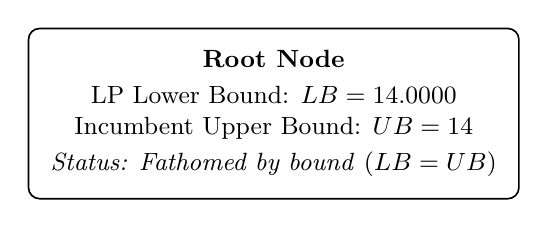
\begin{tikzpicture}[
  every node/.style={
    draw, rounded corners, align=center, font=\small,
    inner sep=8pt, line width=0.6pt
  }
]
\node {%
  \textbf{Root Node}\\[2pt]
  LP Lower Bound: $LB = 14.0000$\\
  Incumbent Upper Bound: $UB = 14$\\[2pt]
  \textit{Status: Fathomed by bound} ($LB = UB$)
};
\end{tikzpicture}
\end{center}

\textbf{Conclusion.}
The branch-and-bound procedure terminates after exploring a single node. The root is
fathomed by bound with $LB=UB=14$, and the optimum $T^*=14$ steps is certified without
any branching. \textbf{Total nodes explored: 1.}

%=======================================================================
\section*{\underline{Question 2: CCI Production Planning}}

\subsection*{Problem Definition}

Coca-Cola \.{I}\c{c}ecek (CCI) plans production at two plants -- Ankara~(A) and
Istanbul~(I) -- over $m=1,\ldots,6$ months. The objective is to minimize the total cost of
inventory holding, cross-region transportation, workforce wages, hiring, layoffs and
bottling mode switching, subject to demand, capacity, workforce and cross shipping
constraints.

\subsection*{Data}

\textbf{Monthly demand} $d_{j,m}$ (liters, L):

\begin{center}
\begin{tabular}{lcccccc}
\toprule
Region $j$ & $m=1$ & $m=2$ & $m=3$ & $m=4$ & $m=5$ & $m=6$ \\
\midrule
Western (W)             & $9{,}000{,}000$ & $9{,}000{,}000$ & $14{,}000{,}000$ & $12{,}000{,}000$ & $12{,}000{,}000$ & $13{,}000{,}000$ \\
Central \& Eastern (CE) & $7{,}000{,}000$ & $7{,}000{,}000$ & $8{,}000{,}000$ & $9{,}000{,}000$ & $8{,}000{,}000$ & $9{,}000{,}000$ \\
\bottomrule
\end{tabular}
\end{center}

\textbf{Plant parameters} ($i\in\{A,I\}$):

\begin{center}
\begin{tabular}{lll}
\toprule
Parameter & Ankara ($i=A$) & Istanbul ($i=I$) \\
\midrule
Bottling rate, 2\,L & $6{,}000$ bot/hr $=12{,}000$ L/hr & $9{,}000$ bot/hr $=18{,}000$ L/hr \\
Bottling rate, 1\,L & $10{,}000$ bot/hr $=10{,}000$ L/hr & $15{,}000$ bot/hr $=15{,}000$ L/hr \\
Available hours/month & 720 & 720 \\
Initial workforce $w_{i,0}$ & 60 & 100 \\
Primary region & CE & W \\
\bottomrule
\end{tabular}
\end{center}

\textbf{Cost parameters:}
\begin{itemize}
  \item Wage: $c_w=1{,}200$ TL/employee/month
  \item Hiring: $c_h=1{,}500$ TL/new employee
  \item Layoff: $c_l=2{,}000$ TL/laid-off employee
  \item Inventory: $c_{\mathrm{inv}}=0.05$ TL/L/month
  \item Cross-region transport: $c_{\mathrm{tr}}=0.10$ TL/L
  \item Switching: $c_{\mathrm{sw}}=20{,}000$ TL/plant/month
\end{itemize}

Policy parameters: $\alpha=0.25$, $\beta=0.10$, $\Delta=10$.

\textbf{Note.} As specified in the project prompt, the demand of every region in every
month is split explicitly into $40\%$ for $1\,$L bottles and $60\%$ for $2\,$L bottles.
Letting $\gamma_1=0.40$ and $\gamma_2=0.60$, the per-size demand is
\[
  d^{1}_{j,m}=\gamma_1\,d_{j,m},\qquad
  d^{2}_{j,m}=\gamma_2\,d_{j,m},\qquad \forall\,j,m,
\]
and these split demands must be fulfilled separately by size in the model.

\subsection*{Decision Variables}

Indices: $i\in\{A,I\}$ plant, $j\in\{W,CE\}$ region, $m\in\{1,\ldots,6\}$ month, and
$k\in\{1\text{L},2\text{L}\}$ bottle size. All production, shipment, and inventory
quantities are in liters (L).

\begin{itemize}
  \item $p^{k}_{i,m}\geq0$ \quad volume of size-$k$ bottles produced at plant $i$ in month $m$
  \item $s^{k}_{i,j,m}\geq0$ \quad volume of size-$k$ bottles shipped from plant $i$ to region $j$ in month $m$
  \item $I^{k}_{i,m}\geq0$ \quad end-of-month inventory of size $k$ at plant $i$ in month $m$
  \item $w_{i,m}\in\mathbb{Z}_{\geq0}$ \quad packaging workforce at plant $i$ in month $m$
  \item $h_{i,m},\,l_{i,m}\in\mathbb{Z}_{\geq0}$ \quad employees hired / laid off
  \item $\delta_{i,k,m}\in\{0,1\}$ \quad 1 if bottle size $k$ is produced at plant $i$ in month $m$
  \item $z_{i,m}\in\{0,1\}$ \quad 1 if both bottle sizes are produced at plant $i$ in month $m$
\end{itemize}

\subsection*{Objective Function}

\[
\min\;Z = C_{\mathrm{inv}}+C_{\mathrm{tr}}+C_w+C_h+C_l+C_{\mathrm{sw}}
\]
\begin{align*}
C_{\mathrm{inv}} &= 0.05\sum_{i}\sum_{m}\sum_{k}I^{k}_{i,m} \\
C_{\mathrm{tr}}  &= 0.10\!\!\!\sum_{\substack{i,j:\,j\neq\mathrm{primary}(i)}}\sum_{m}\sum_{k}s^{k}_{i,j,m} \\
C_w  &= 1{,}200\sum_{i}\sum_{m}w_{i,m} \\
C_h  &= 1{,}500\sum_{i}\sum_{m}h_{i,m} \\
C_l  &= 2{,}000\sum_{i}\sum_{m}l_{i,m} \\
C_{\mathrm{sw}} &= 20{,}000\sum_{i}\sum_{m}z_{i,m}
\end{align*}

\subsection*{Constraints}

\textbf{(D1) Bottling capacity} (hours $\leq720$ per plant per month):
\[
  \frac{p^2_{A,m}}{12{,}000}+\frac{p^1_{A,m}}{10{,}000}\leq720,
  \qquad
  \frac{p^2_{I,m}}{18{,}000}+\frac{p^1_{I,m}}{15{,}000}\leq720
  \qquad\forall\,m
\]

\textbf{(D2) Packaging capacity:}
\[
  p^1_{i,m}+p^2_{i,m}\leq100{,}000\,w_{i,m} \qquad\forall\,i,m
\]

\textbf{(D3) Workforce balance} ($w_{A,0}=60$, $w_{I,0}=100$):
\[
  w_{i,m}=w_{i,m-1}+h_{i,m}-l_{i,m} \qquad\forall\,i,m
\]

\textbf{(D4) Workforce smoothing} ($\Delta=10$):
\[
  w_{i,m}-w_{i,m-1}\leq10, \qquad w_{i,m-1}-w_{i,m}\leq10 \qquad\forall\,i,m
\]

\textbf{(D5) Inventory balance} (initial inventories $I^{k}_{i,0}=0$), per bottle size:
\[
  I^{k}_{i,m}=I^{k}_{i,m-1}+p^{k}_{i,m}-\sum_{j}s^{k}_{i,j,m}
  \qquad\forall\,i,m,k
\]

\textbf{(D6) Demand fulfillment} (no backlogging), per bottle size:
\[
  \sum_{i}s^{k}_{i,j,m}\;=\;\gamma_k\,d_{j,m}
  \qquad\forall\,j,m,k,
\]
with $\gamma_1=0.40$ and $\gamma_2=0.60$.

\textbf{(D7) Perishability} (inventory cannot be carried for more than one month;
since $I^{k}_{i,0}=0$, this reduces to: end-of-month inventory cannot exceed the
production of that same month):
\[
  I^{k}_{i,m}\;\leq\;p^{k}_{i,m} \qquad\forall\,i,m,k
\]

\textbf{(D8) Cross-shipping cap} ($\alpha=25\%$):
\[
  \sum_{k}s^{k}_{i,j,m}\;\leq\;\alpha\,d_{j,m}
  \qquad\forall\,i,m,\;j\neq\mathrm{primary}(i)
\]

\textbf{(D9) Safety stock} ($\beta=10\%$, months $m=1,\ldots,5$):
\[
  \sum_{k}I^{k}_{i,m}\;\geq\;\beta\,d_{j^*(i),\,m+1}
  \qquad m=1,\ldots,5,
\]
where $j^*(i)$ is the primary region of plant $i$.

\textbf{(D10) Zero ending inventory:}
\[
  I^{k}_{i,6}=0 \qquad\forall\,i,k
\]

\textbf{(D11) Switching cost} (big-$M=50{,}000{,}000$ L):
\[
  p^k_{i,m}\leq50{,}000{,}000\,\delta_{i,k,m} \qquad\forall\,i,k,m
\]
\[
  z_{i,m}\geq\delta_{i,1\mathrm{L},m}+\delta_{i,2\mathrm{L},m}-1 \qquad\forall\,i,m
\]

\end{document}
